\section{Runtime Example}

\begin{frame}{Runtime Example}
  \begin{figure}[!h]
    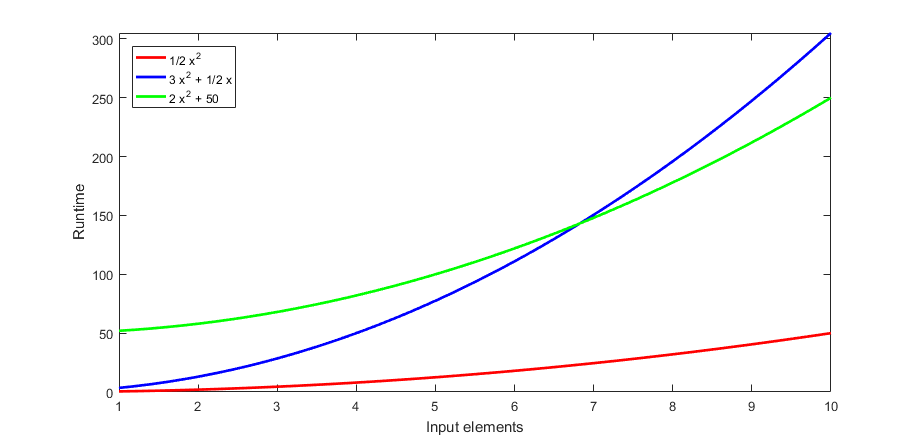
\includegraphics[width=\linewidth]
      {Lecture/Images/Runtime/SquaredRuntime.png}%
    \caption{Different functions with quadratic runtime}%
    \label{fig:squared_runtime}%
  \end{figure}
\end{frame}

%-------------------------------------------------------------------------------

\begin{frame}{Runtime Example}
  \begin{itemize}
    \item
      The runtime is growing quadratic with the number of elements
      ${\color{Mittel-Blau}n}$ in the list.\\
    \item
      $2\, \times$ elements $\Rightarrow$ $4\, \times$ runtime\\
      \begin{itemize}
        \item 
          $C = \SI{1}{\nano\second}$
          (1 simple instruction $\approx \SI{1}{\nano\second}$)
        \item 
          $n = 10^6$ (1 million numbers = $\SI{4}{\mega\byte}$
          with $\SI{4}{\byte\per number}$)
          \begin{itemize}
            \item 
              $C \cdot n^2 = \SI{e-9}{\second} \cdot 10^{12}
               = \SI{e3}{\second} = \SI{16.7}{\minute}$
          \end{itemize}
        \item 
          $n = 10^9$ (1 billion numbers = $\SI{4}{\giga\byte}$)
          \begin{itemize}
            \item 
              $C \cdot n^2 = \SI{e-9}{\second} \cdot 10^{18}
               = \SI{e9}{\second} = 31.7$~years
          \end{itemize}
      \end{itemize}
    \item
      \textbf{Quadratic runtime = \enquote{big} problems unsolvable}
  \end{itemize}
\end{frame}